\subsection{Conduct DNSSEC monitoring}
\label{section:conduct-dnssec-monitoring}
To present how monitoring can be conducted using our created MIB, an example use case is sketched. To implement the monitoring tasks, the well known monitoring system Nagios \cite{nagios} and its SNMP plugin \textit{check-snmp} \cite{check-snmp} is used.
%%\textit{check_snmp}      %%\cite{check_snmp} is used. 
\\
Assuming the RRSIG RR of the SOA record and the DNSKEY RR (KSK) of the DNSSEC signed zone \textit{paris.derby.practicum.os3.nl} have expired. That will lead an DNSSEC-aware resolver to invalidate a complete zone. A DNSSEC-aware resolver will only return a \textit{SERVFAIL} without specifying the root cause for invalidation itself when it is queried for RR of that zone. In that case, querying the corresponding OIDs using our MIB might be helpful. Values for the object-type \textit{ dnssecZoneGlobalServFail} will return an error (2) but also the validation check \textit{dnssecZoneGlobalDNSKEYSignatureVerification} in table \textit{dnssecZoneGlobalTable} will return an error (2) for that zone. 
\\
The actual reason for the \textit{SERVFAIL} can be derived from table \textit{ dnssecZoneSigTable}, in particular from object-type \textit{ dnssecZoneSigDNSKEYSignatureExpirationTime}. It will show a expired date for that RRSIG, in that case the expiration of the RRSIG occurred on 27th of January 2015 on 19:50:10. Figure \ref{figure:nagios} shows the applied Nagios implementation.

\begin{figure}[H]
\centering
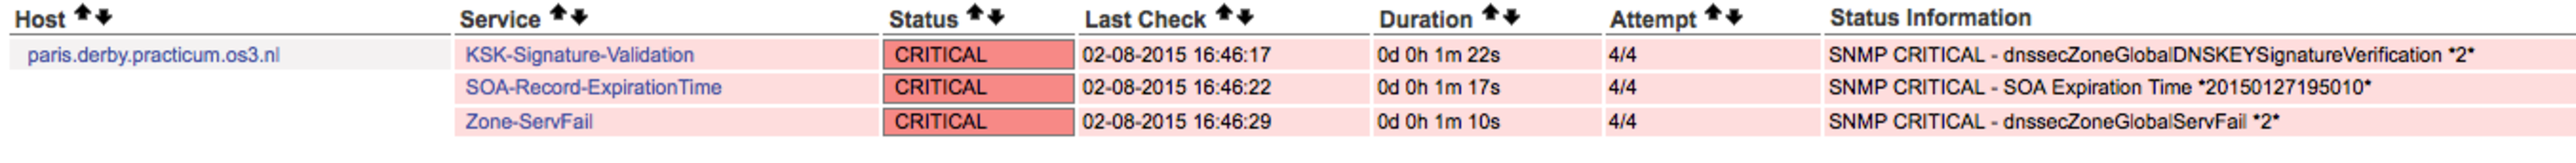
\includegraphics[scale=0.3]{Images/nagios.pdf}
\caption{implemented Nagios checks based on values of the DNSSEC-MIB}
\label{figure:nagios}
\end{figure}
 
